\section{Première modélisation abstraite}
	
%\subsection{}
%\paragraph{}

   On veut initialement considérer très peu d'exigences. L'énoncé nous indique
   que seules les entrées et sorties de l'aéroport sont étudiées. On effectue donc une étude formelle sur un système très simplifié où la piste et le tarmac ne sont pas pris en compte. Nous étudions uniquement les échanges d'avions entre l'aéroport et l'extérieur ce qu'on modélise en utilisant deux events ou transitions :
   
   \begin{itemize}
   	\item extout lorsqu'un avion sort de l'espace extérieur pour rentrer dans l'espace aéroportuaire,
   	\item extin lorsqu'un avion entre dans l'espace extérieur.
   \end{itemize} 

\begin{figure}[H]
	\begin{center}	
		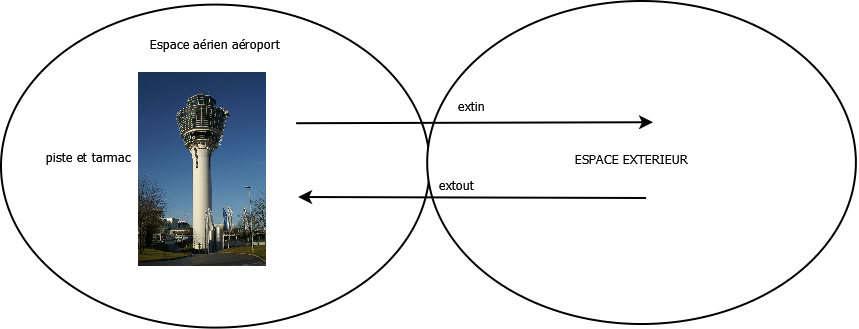
\includegraphics[scale=0.4]{images/mod0}
		\caption{Modèle abstrait}
		\label{mod0}
	\end{center}
\end{figure}

On fait abstraction de la piste. Ainsi, la seule variable à considérer est le nombre d'avions présents sur le tarmac à un instant donné. On note nt cette variable.

\paragraph{Etat static ou \textit{contexte} du système :}
L'état statique est caractérisé par ntmax :
\begin{figure}[H]
	\begin{center}	
		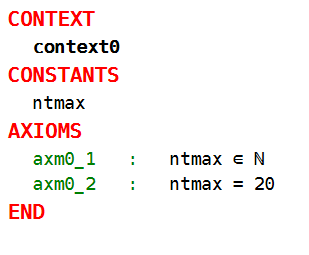
\includegraphics[scale=0.8]{images/ctx0}
		\caption{Etat static du système}
		\label{ctx0}
	\end{center}
\end{figure}

\paragraph{Etat dynamique du système :}
 L'état dynamique du système n'est constitué que de cette seule variable. Elle est définie au moyen de deux conditions ou \textit{invariants} :
%   \begin{align}
%  inv0\_1 : nt \in ℕ 
%   \end{align}
%   
%    \begin{align}
%   inv0\_2 : nt \le ntmax
%   \end{align}
%   

\begin{figure}[H]
	\begin{center}	
		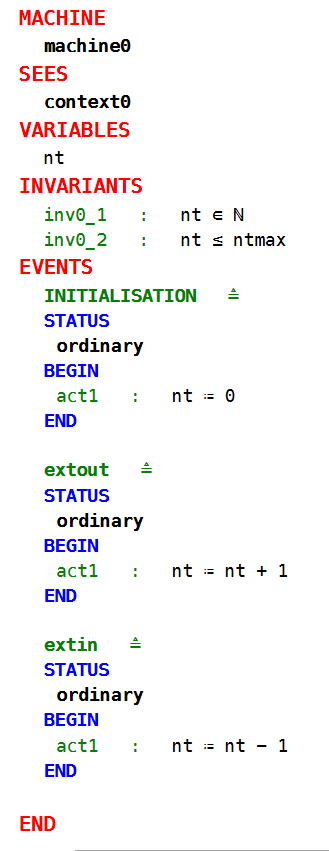
\includegraphics[scale=0.8]{images/mac0}
		\caption{Etat dynamique du système}
		\label{mac0}
	\end{center}
\end{figure}


